\documentclass[11pt]{article}
\usepackage{amsmath}
\usepackage{physics}
\usepackage{amssymb}
\usepackage{graphicx}
\usepackage{hyperref}
\usepackage{amsfonts}
\usepackage{cancel}
\usepackage{xcolor}
\hypersetup{
	colorlinks,
	linkcolor={black!50!black},
	citecolor={blue!50!black},
	urlcolor={blue!80!black}
}
\usepackage{newpxtext,newpxmath}
\usepackage[left=1.25in,right=1.25in,top=0.9in,bottom=0.9in]{geometry}


%\newcommand{\fig}[1]{figure #1}
%\newcommand{\explain}{appendix?}
%\newcommand{\rat}{\mathbb{Q}}
%
%\newcommand{\mathbb{R}}{\mathbb{R}}
%\newcommand{\nat}{\mathbb{N}}
%\newcommand{\inte}{\mathbb{Z}}
%\newcommand{\M}{{\cal{M}}}
%\newcommand{\sss}{{\cal{S}}}
%\newcommand{\rrr}{{\cal{R}}}
%\newcommand{\uu}{2pt}
%\newcommand{\vv}{\vec{v}}
%\newcommand{\comp}{\mathbb{C}}
%\newcommand{\field}{\mathbb{F}}
%\newcommand{\f}[1]{ \hspace{.1in} (#1) }
%\newcommand{\set}[2]{\mbox{$\left\{ \left. #1 \hspace{3pt}
%\right| #2 \hspace{3pt} \right\}$}}
%\newcommand{\integral}[2]{\int_{#1}^{#2}}
%\newcommand{\ba}{\hookrightarrow}
%\newcommand{\ep}{\varepsilon}
%\newcommand{\limit}{\operatornamewithlimits{limit}}
%\newcommand{\ddd}{.1in}
%\newcommand{\ccc}{2in}
%\newcommand{\aaa}{1.5in}
%\newcommand{\B}{{\cal B}}
%\newcommand{\C}{{\cal C}}
%\newcommand{\D}{{\cal D}}
%\newcommand{\FF}{{\cal F}}


%\usepackage{epstopdf}
%\DeclareGraphicsRule{.tif}{png}{.png}{`convert #1 `basename #1 .tif`.png}
%\usepackage{graphics}
%\usepackage{array}
%\def\set#1#2{\left\{\left.\;#1\;\right| #2 \; \right\}}
%\def\Sum{\sum}
%\def\me{.05in}















\begin{document}
\begin{center}
{\large \bf PH312: Physics of Fluids (Prof. McCoy) -- Informal Reflection}\\
{ Huan Q. Bui}\\
Feb 18, 2021
\end{center}

\noindent So far, we have covered three simple examples in fluid dynamics:
\begin{enumerate}
	\item Simple shear flows in channels and pipes
	\item Flow around an obstacle (cylinder)
	\item Pattern formation in fluids heated from below.
\end{enumerate}

While I have heard of these phenomena (from PH333 and other experiences), they never quite cease to be mysterious to me. I think this is because I interact with fluids (air, water, etc.) so constantly that I simply don't associate ``complex physics'' with them, whereas I grew up learning that quantum physics is ``strange'' and ``counter-intuitive'' and so the sense of mystery there is not as strong. \\

I want to first comment a bit on the introduction of dimensionless quantities such as the Reynolds number and the Rayleigh number. I think that this feature of fluids dynamics (as far as I know) is really unique because it means that different parts of a fluid-dynamical system might not scale the ``usual'' way with respect to the system size in order to preserve its behavior. For example, we can easily make a fluid-dynamical system in laminar flow go turbulent in its 2:1 model. This is very much unlike Newtonian kinematics, where an elastic collision between two objects of mass $m$ traveling at velocities $v$ and $-v$ is exactly the same as that between two objects of mass $2m$ traveling at velocities $2v$ and $-2v$. As a result, I can imagine that constructing functional and safe hydrodynamics structures such as dams, reservoirs, etc. can be very challenging for engineers because they will have to figure out how to appropriately scale up their models without compromising the integrity of their designs. \\
 
I also find the experimental side of things very subtle because of how simple yet revealing some of the experiments we have seen can be: Only from the specific conditions such as pipes/channels/laminar flow around a cylinder/etc. were scientists able to deduce the seemingly simple laws for fluid motion (e.g. Poiseuille's law). I feel that for most of the past, scientists had been very interested in and had some intuition for fluid dynamics, but could not deduce these laws for flow. Without the mathematics and necessary experimental methods, a lot of investigations (especially of complex phenomena such as vortex dynamics), which date back to antiquity, had been mostly qualitative -- which is how  I believe most of us feel about fluids dynamics since we aren't formally introduced to the topic. Everybody seems to find it very fascinating (some even make a career out of capturing fluid motion in various forms of paintings/pottery/bartending/etc.), but no one really understands the mechanism governing such motion unless they conduct careful experiments in highly idealized scenarios. So, I think that even coming up with the idea of observing fluid motion in a tight gap between two sheets of glass in order to make some generalizations about how it might general behave, say, in a large tank heated from below is already ingenious. 


\begin{figure}[!htb]
	\centering
	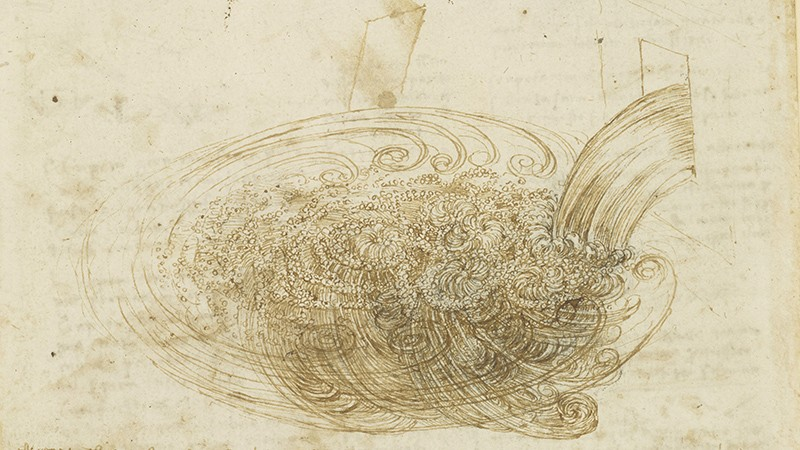
\includegraphics[scale=0.5]{davinci}
	\caption{da Vinci's sketch of turbulent water. He was one of the first to methodically setup experiments and record various interesting behaviors of water. Credit: Leonardo da Vinci, Studies of Turbulent Water, Royal Collection Trust}
	\label{fig:davinci}
\end{figure} 

\begin{figure}[!htb]
	\centering
	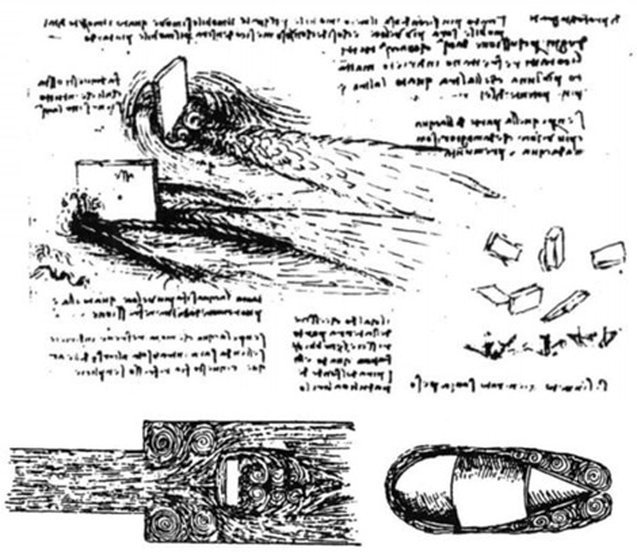
\includegraphics[scale=0.5]{davinci_1}
	\caption{Another of da Vinci's extensive collection of highly detailed fluid mechanical drawings. Here, he's sketching the flow of water around various obstacles.}
	\label{fig:davinci1}
\end{figure} 

  
\end{document}




